\documentclass[12pt, a4paper]{article}
\usepackage{ctex} % 支持中文处理
\usepackage{geometry} % 页面布局
\usepackage{graphicx} % 图片支持
\usepackage{subcaption}
\usepackage{hyperref} % 超链接支持
\usepackage{amsmath} % 数学公式
\usepackage{amsfonts}
\usepackage{amssymb}
\usepackage{amsthm}
\usepackage{bm}
\usepackage{color}

\geometry{left=2.5cm,right=2.5cm,top=2.5cm,bottom=2.5cm} % 设置页边距
\title{结果讨论}
\author{安庭毅\ 工学院 \ 2100011014}
\date{\today} % 使用今天的日期

\begin{document}

\maketitle % 显示标题
\section{格式精度验证}
根据数理算法原理部分的算法推导,计算得到的精度阶数如下图所示(采取函数为$\sin x$,计算点为$x=1$):

\begin{figure}[htbp]
    \centering
    \begin{subfigure}[b]{0.45\textwidth} 
        \centering
        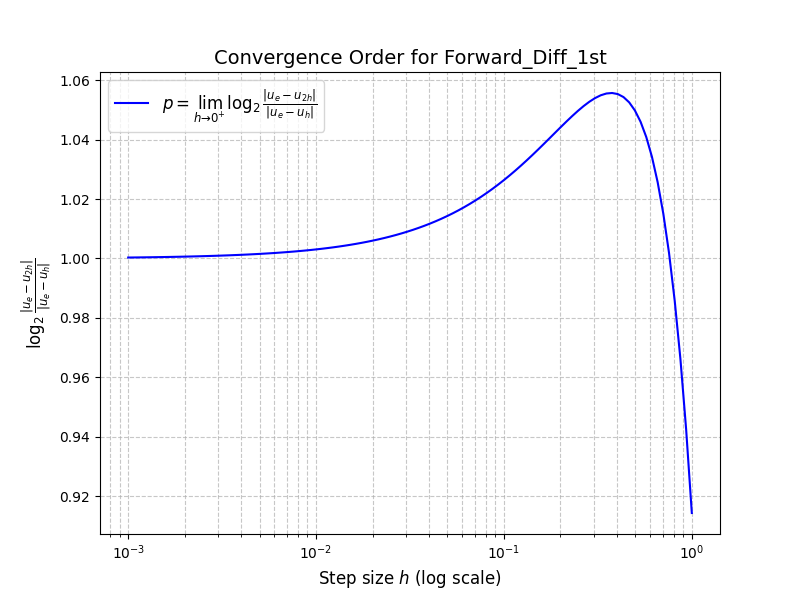
\includegraphics[width=\textwidth]{./pictures/Convergence Order for Forward_Diff_1st.png} 
        \caption{一阶导数的向前差分精度}
        \label{fig: COF1}
    \end{subfigure}
    \hfill
    \begin{subfigure}[b]{0.45\textwidth} 
        \centering
        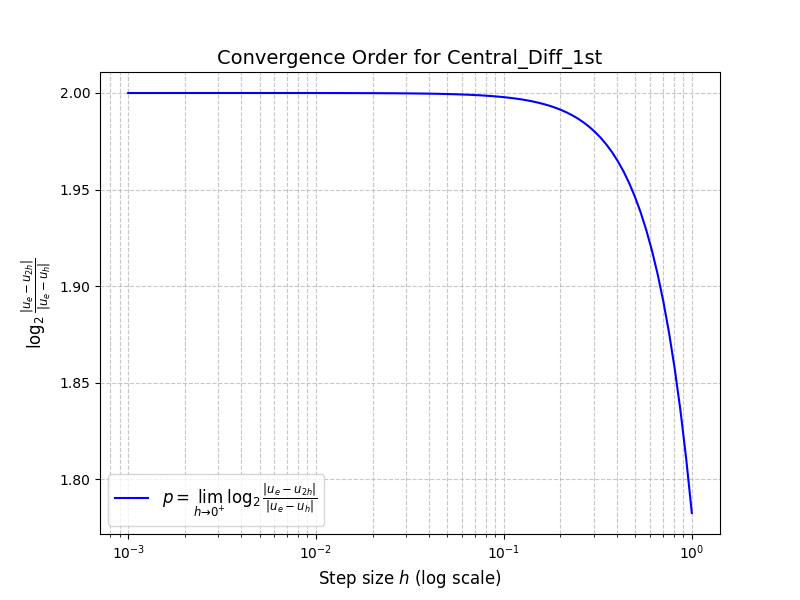
\includegraphics[width=\textwidth]{./pictures/Convergence Order for Central_Diff_1st.png} 
        \caption{一阶导数的中心差分精度}
        \label{fig: COC1}
    \end{subfigure}
    \vspace{0.5cm}
    \centering
    \begin{subfigure}[b]{0.45\textwidth} 
        \centering
        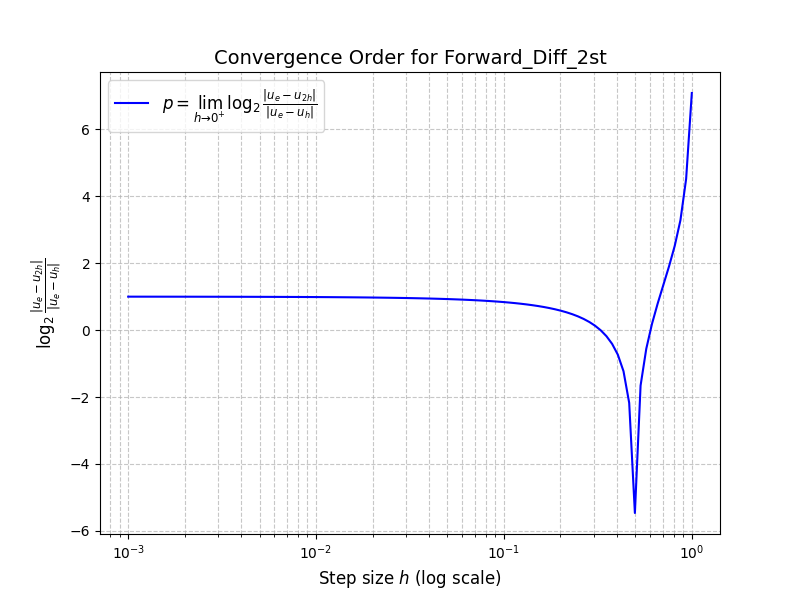
\includegraphics[width=\textwidth]{./pictures/Convergence Order for Forward_Diff_2st.png} 
        \caption{二阶导数的向前差分精度}
        \label{fig: COF2}
    \end{subfigure}
    \hfill
    \begin{subfigure}[b]{0.45\textwidth} 
        \centering
        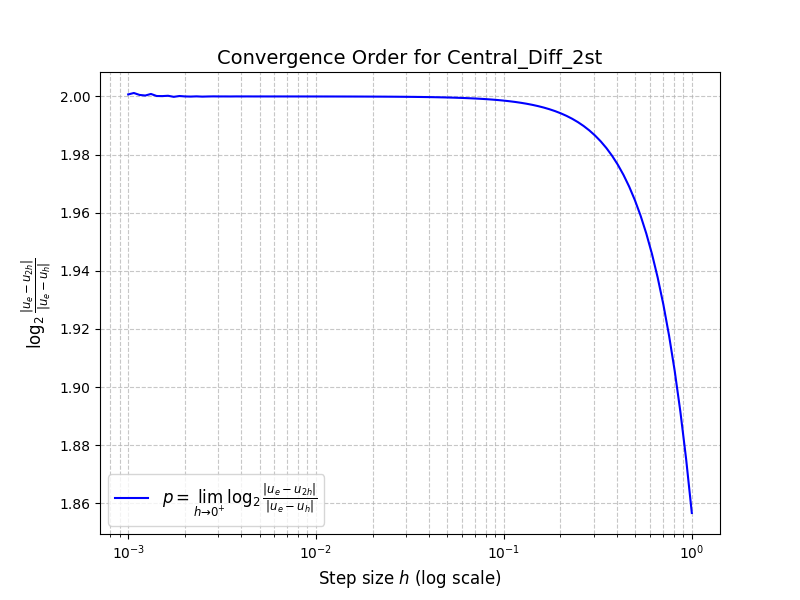
\includegraphics[width=\textwidth]{./pictures/Convergence Order for Central_Diff_2st.png} 
        \caption{二阶导数的中心差分精度}
        \label{fig: COC2}
    \end{subfigure}
\end{figure}

可以看到,随步长减少,公式收敛到的结果与理论推导得到的精度一致。
以上计算均使用双精度,注意到二阶导数的中心差分精度阶在步长极小的情况下已经出现了由于舍入误差带来的波动。

\section{截断误差与舍入误差分析}
下图为分别针对多项式和$\sin x$计算导数得到的误差随步长变化,均采用双精度,步长和误差均取对数展示:
\begin{figure}[htbp]
    \centering
    \begin{subfigure}[b]{0.45\textwidth} 
        \centering
        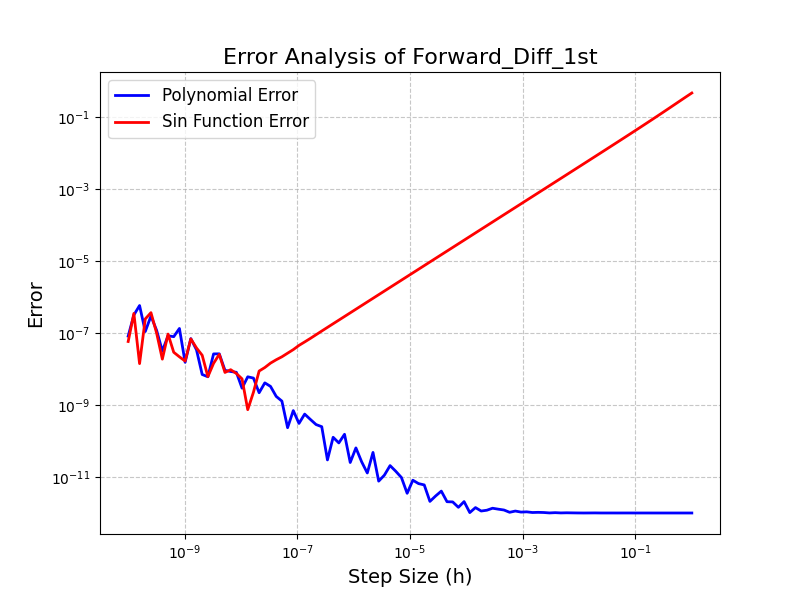
\includegraphics[width=\textwidth]{./pictures/Error Analysis of Forward_Diff_1st.png} 
        \caption{一阶导数的向前差分误差:$\sin x$和$x$}
        \label{fig: EAF1}
    \end{subfigure}
    \hfill
    \begin{subfigure}[b]{0.45\textwidth} 
        \centering
        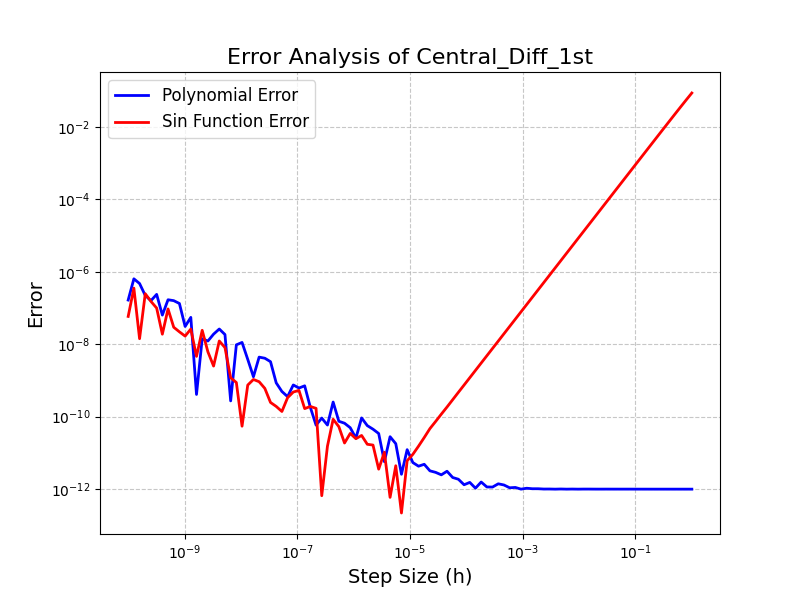
\includegraphics[width=\textwidth]{./pictures/Error Analysis of Central_Diff_1st.png} 
        \caption{一阶导数的中心差分误差:$\sin x$和$x^2$}
        \label{fig: EAC1}
    \end{subfigure}
    \vspace{0.5cm}
    \centering
    \begin{subfigure}[b]{0.45\textwidth} 
        \centering
        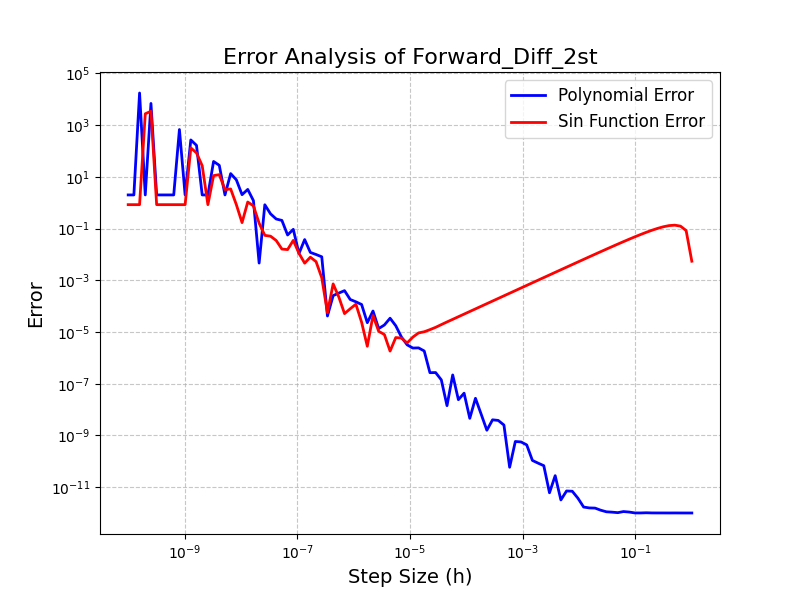
\includegraphics[width=\textwidth]{./pictures/Error Analysis of Forward_Diff_2st.png} 
        \caption{二阶导数的向前差分误差:$\sin x$和$x^2$}
        \label{fig: EAF2}
    \end{subfigure}
    \hfill
    \begin{subfigure}[b]{0.45\textwidth} 
        \centering
        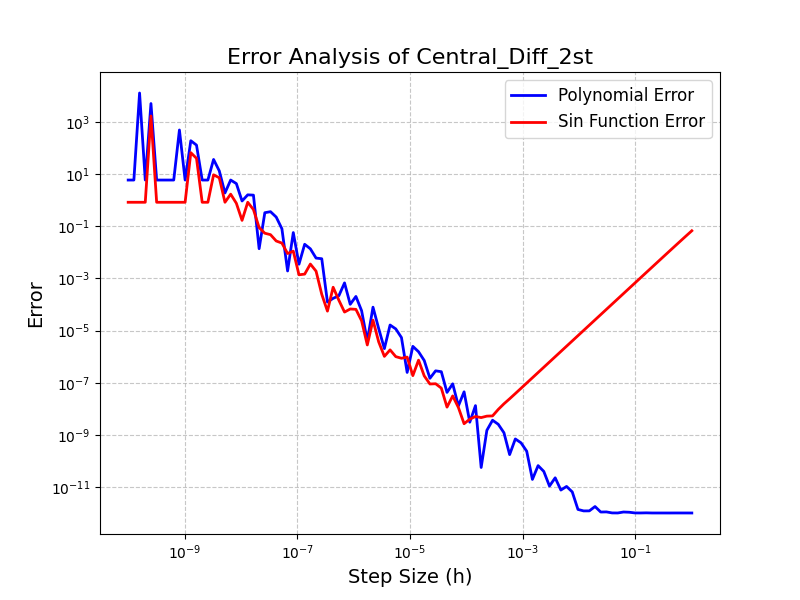
\includegraphics[width=\textwidth]{./pictures/Error Analysis of Central_Diff_2st.png} 
        \caption{二阶导数的中心差分误差:$\sin x$和$x^3$}
        \label{fig: EAC2}
    \end{subfigure}
\end{figure}

在测试时,为避免多项式计算的截断误差为0导致取对数后带来计算错误,为总误差加上小量$1e-12$。
由于在舍入误差占主导时这小量造成影响可以忽略,因此反应的变化趋势仍是合理的。

可以看到,对于采用的多项式函数,在步长减小到一定程度后舍入误差开始占主导,浮点运算带来的误差
随步长减小逐渐增大。而对于采用的$\sin x$,在步长较长时,取对数后步长和误差呈线性关系,这是由于截断误差占主导,
根据上一节的分析,截断误差与步长的$p$次方之比接近常数,取对数后自然为一直线。另外,注意到中心差分的直线斜率大于
向前差分,这也说明了中心差分的精度阶数更高。而随着步长减小,舍入误差开始占主导,总误差由于步长减小带来的舍入误差而增大。

注意到对于采用的多项式函数,其舍入误差开始主导的步长均大于正弦函数,这应该是由于指数运算带来的精度误差高于numpy的正余弦
函数。在进入舍入误差主导的步长范围后,总误差与步长取对数后又接近线性关系,且选取的不同计算函数表现出的舍入误差基本一致。
这应该是由于舍入误差开始占主导后主要取决于格式的浮点运算次数。

\section{单双精度误差对比}
下给出各差分格式的单双精度计算结果随步长的变化,仍取对数(均采用$\sin x$为测试函数,计算点为$x=1$):
\begin{figure}[htbp]
    \centering
    \begin{subfigure}[b]{0.45\textwidth} 
        \centering
        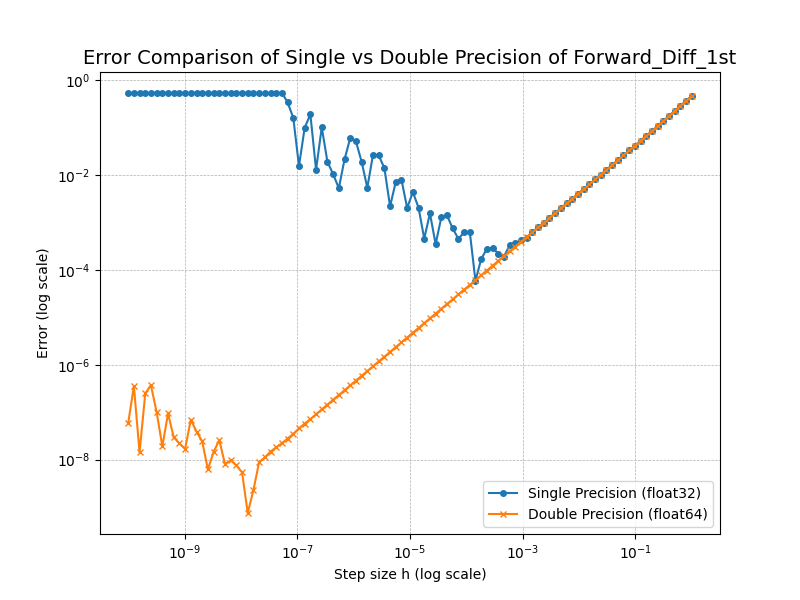
\includegraphics[width=\textwidth]{./pictures/Error Comparison of Single vs Double Precision of Forward_Diff_1st.png} 
        \caption{一阶导数的向前差分误差:单双精度}
        \label{fig: ECCF1}
    \end{subfigure}
    \hfill
    \begin{subfigure}[b]{0.45\textwidth} 
        \centering
        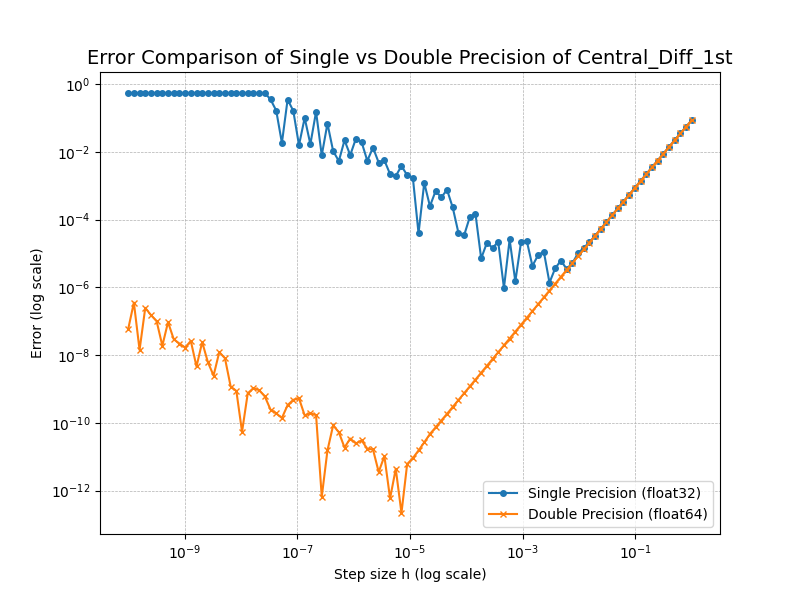
\includegraphics[width=\textwidth]{./pictures/Error Comparison of Single vs Double Precision of Central_Diff_1st.png} 
        \caption{一阶导数的中心差分误差:单双精度}
        \label{fig: ECC1}
    \end{subfigure}
    \vspace{0.5cm}
    \centering
    \begin{subfigure}[b]{0.45\textwidth} 
        \centering
        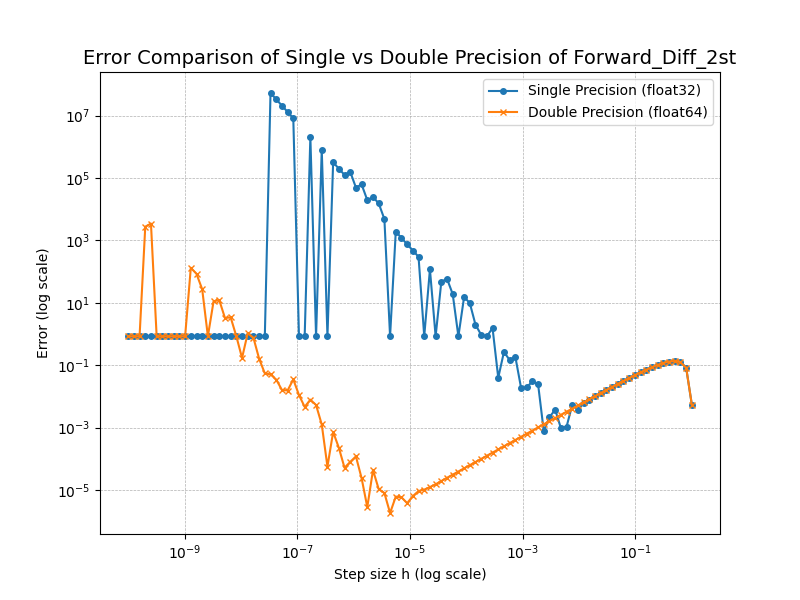
\includegraphics[width=\textwidth]{./pictures/Error Comparison of Single vs Double Precision of Forward_Diff_2st.png} 
        \caption{二阶导数的向前差分误差:单双精度}
        \label{fig: ECF2}
    \end{subfigure}
    \hfill
    \begin{subfigure}[b]{0.45\textwidth} 
        \centering
        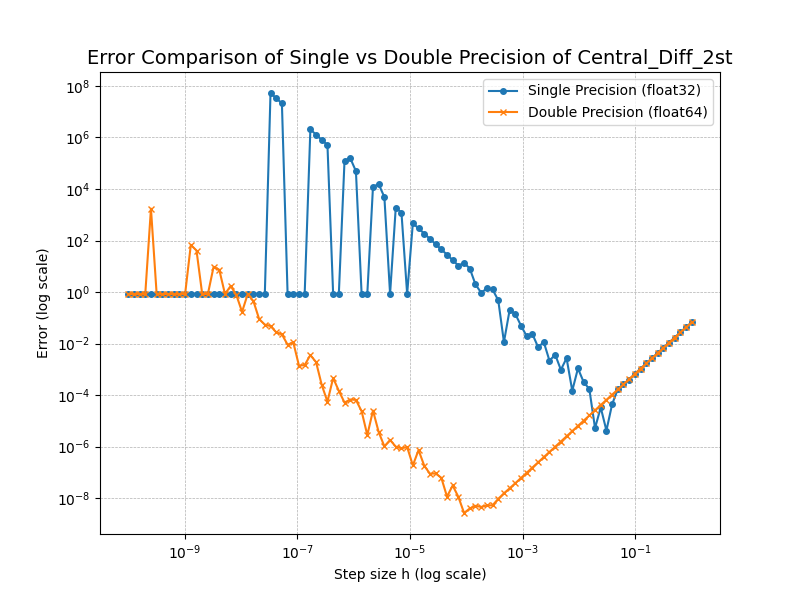
\includegraphics[width=\textwidth]{./pictures/Error Comparison of Single vs Double Precision of Central_Diff_2st.png} 
        \caption{二阶导数的中心差分误差:单双精度}
        \label{fig: ECC2}
    \end{subfigure}
\end{figure}

可以看出,精度主要影响舍入误差。随步长减小,单精度总误差要比双精度更快由舍入误差主导。
\end{document}